% energy.tex
% $Author$ $Date$

% Predrag                   Apr 12 2007

\subsection{Energy budget} % of the \KSe}
\label{sec:energy}

% Predrag                   mar 13 2007
\PC{
from bounds on energy, we might be able
to bound the number of equilibria as function of systems size $L$, and thus
be sure we have them all.
   }
%
The {space average} of a function $\obser = \obser(\pSpace,t)$  on
the interval $L$,
\beq
    \expct{\obser} = \frac{1}{L}\int_0^{L} d\pSpace\, \obser(\pSpace,t)
    \,,
    \label{rpo:spac_ave}
\eeq
is in general time dependent. 
Its mean value is given by the {time average}
\beq
\timeAver{\obser}
    =
\lim_{t\rightarrow \infty} {1\over t} \int_0^t \! d\tau \, \expct{\obser}
    =
\lim_{t\rightarrow \infty} {1\over t L} \int_0^t \! 
    \int_0^{L} \!\! d\tau  d\pSpace\, \obser(\pSpace,\tau)
    \,.
\label{rpo:tim_ave}
\eeq
The mean value
$\timeAver{\obser}$, $\obser = \obser(u)$ evaluated on an
\eqv\ or {\reqv} $u(\pSpace,t) = u_q(\pSpace-ct)$ is
\beq
         \obser_q = \expct{\obser}_q
\,.
\label{rpo:u-eqv}
\eeq
Evaluation of the infinite time average \refeq{rpo:tim_ave}
on a function of a period $\period{p}$
\po\ or \rpo\ $u_p(\pSpace,t)$
 requires only a single traversal of the periodic solution,
\beq
       \obser_p = \frac{1}{\period{p}}
    \int_0^{\period{p}} \! d\tau \, \expct{\obser}
\,.
\label{rpo:u-cyc}
\eeq

Equation \refeq{ks} can be written as % in ``potential'' form
\beq
    u_t=- V_x
        \,,\qquad
    V(x,t)={\textstyle\frac{1}{2}}u^2+u_{x} + u_{xxx}
    \,.
\ee{ksPotent}
$u$ is related to the ``flame-front height'' $h(x,t)$ by
$u=h_x$, so \expctE\ can be interpreted as
the mean energy density \refeq{ksEnergy}.

Even though KS is a phenomenological
small-amplitude model equation, the time-dependent quantity
\beq
    \expctE=\frac{1}{L}\int_0^{L} \!dx \, V(x,t)
    =\frac{1}{L}\int_0^{L}\! dx \, \frac{u^2}{2}
\label{ksEnergy}
\eeq
% \PC{this is missing a prefactor 1/2. Check if someone in literature
% - other than Greene and Kim - defines it right. }
has a physical interpretation\rf{ksgreene88}
as the average ``energy'' density of the flame front.
This analogy to the corresponding definition of the
mean kinetic energy density for
the Navier-Stokes will be useful in what follows.
\PC{bit weird: can use Galilean invariance to
    set $\expctE=0$ for any given $u(x,t)$?}

The energy \refeq{ksEnergy}
is also the quadratic norm in the Fourier space,
\beq
\expctE   % = (u,u) 
          = \sum_{k=1}^{\infty} E_k
\,,\qquad
E_k = % a_{-k} a_k =
    {\textstyle\frac{1}{2}}|a_k|^2
\,.
\ee{EFourier}

Take time derivative of the energy density \refeq{ksEnergy},
substitute \refeq{ks} and integrate by parts. Total derivatives vanish
by the spatial periodicity on the $L$ domain:
\bea
   \dot{\expctE} &=&
     \expct{u_t \, u}
    % \frac{1}{L}\int_0^{L}u \, u_t\, dx
     = - \expct{(\frac{u^2}{2} + u \, u_{x} + u \, u_{xxx})_x u }
    \continue
    &=&
\expct{+ u_x \, \frac{u^2}{2} + (u_{x})^2 + u_x \, u_{xxx}}
    \,.
\label{rpo:ksErate}
\eea
Substitution by \refeq{KSeqvCond}
verifies that for an \eqv\ $\expctE$ is constant:
\[
   \dot{\expctE} =
\expct{ \left(\frac{u^2}{2} + u_{x} + u_{xxx} \right) \,u_x}
    = \expctE \expct{ u_x }=0
    \,.
\]
The first term in \refeq{rpo:ksErate} vanishes by
integration by parts,
\(
 \expct{(u^3)_x} = 3 \expct{ u_x \, u^2}=0
\,,
\) % {EnNonl0}
and integrating the third term by parts yet again we get
that the energy variation
% \PC{this is ``power", nicht war?}
\beq
   \dot{\expctE} =
      \expct{(u_{x})^2} - \expct{(u_{xx})^2}
\ee{EnRate}
balances the KS equation \refeq{ks} power pumped in by the anti-diffusion
$u_{xx}$
against energy dissipated by the hypervicosity $u_{xxxx}$ \rf{ksgreene88}.

%%%%%%%%%%%%%%%%%%%%%%%%%%%%%%%%%%%%%%%%%%%%%%%%%%%%%%%%%%%%%%%%
\begin{figure}[t] 
\begin{center}
    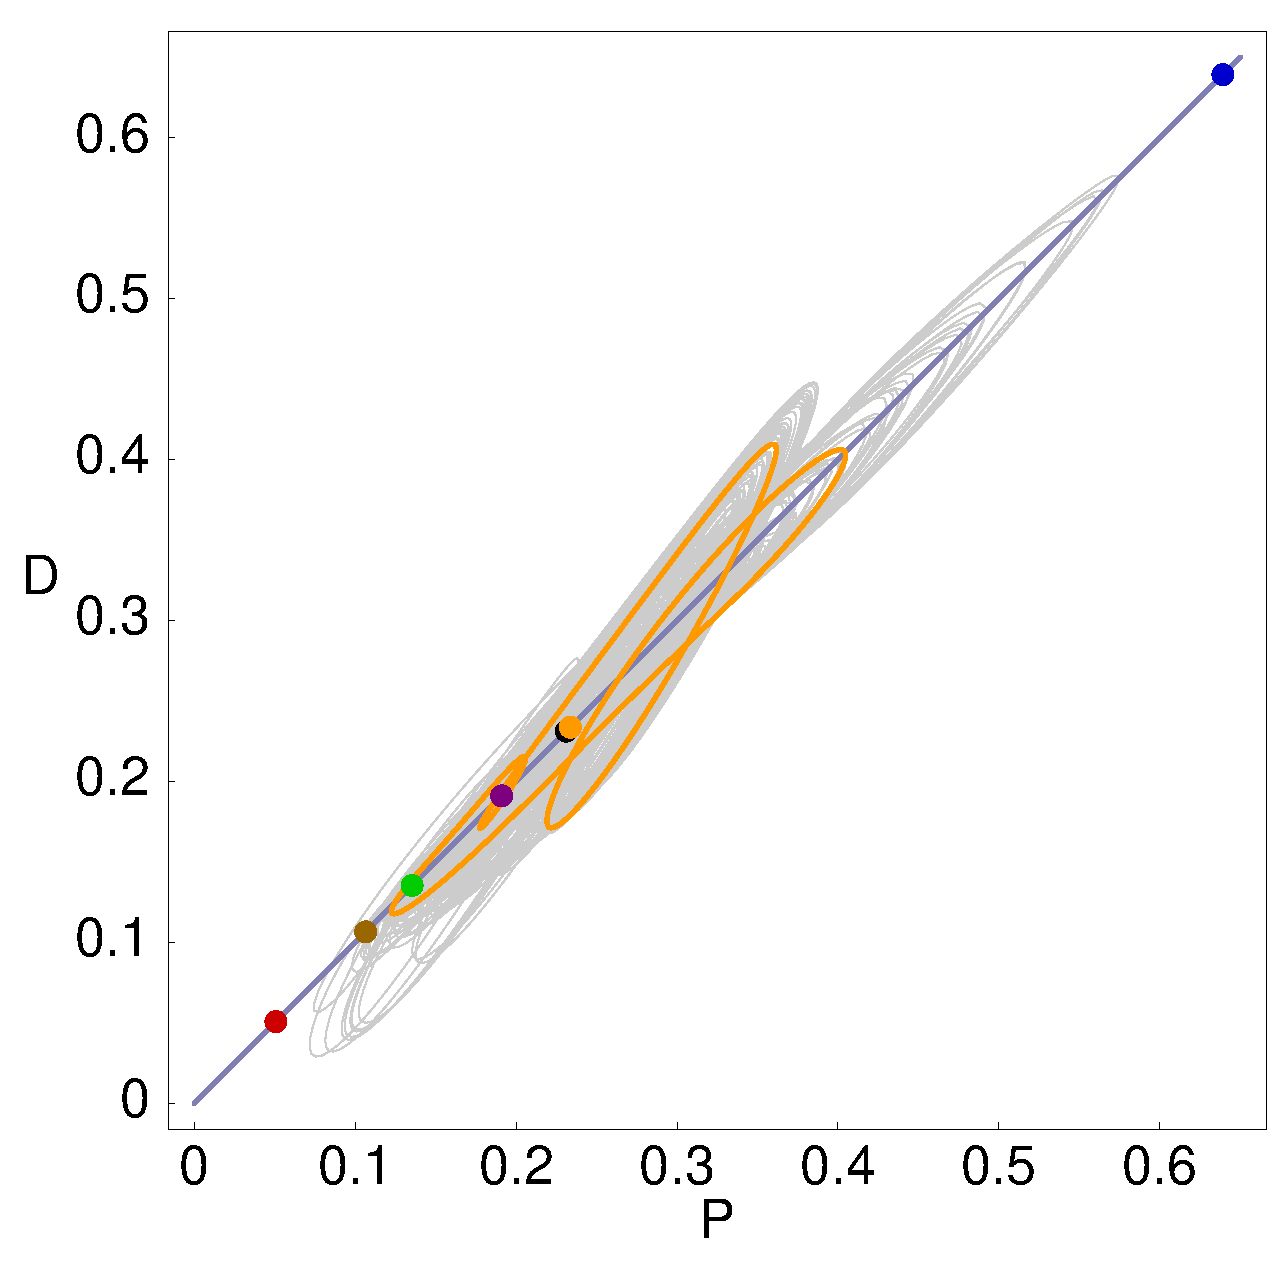
\includegraphics[width=\textwidth]{figs/energyBalancePlot.eps}
\end{center}
\caption{
Power input $\expct{(u_{x})^2}$ vs.
dissipation $\expct{(u_{xx})^2}$ for $L=22$ \eqva\
and \reqva, for several
% \ESedit{(two, more in the way!)}
\po s and \rpo s, and for a typical ``turbulent"
state. Note that $\timeAver{(u_{p,x})^2}$
of the
$(\period{p},\shift_p) =(32.8,10.96)$
 {\rpo}, \reffig{f:ks22rposShort}(c), which appears well embedded
within the turbulent state, is close to the turbulent
expectation $\timeAver{(u_x)^2}$
\PCedit{[temporary Japanese heresy]}.
        }
\label{f:drivedrag}
\end{figure}
%%%%%%%%%%%%%%%%%%%%%%%%%%%%%%%%%%%%%%%%%%%%%%%%%%%%%%%%%%%%%%%%%%

%%%%%%%%%%%%%%%%%%%%%%%%%%%%%%%%%%%%%%%%%%%%%%%%%%%%%%%%%%%%%%%%
\begin{figure}[t] 
\begin{center}
    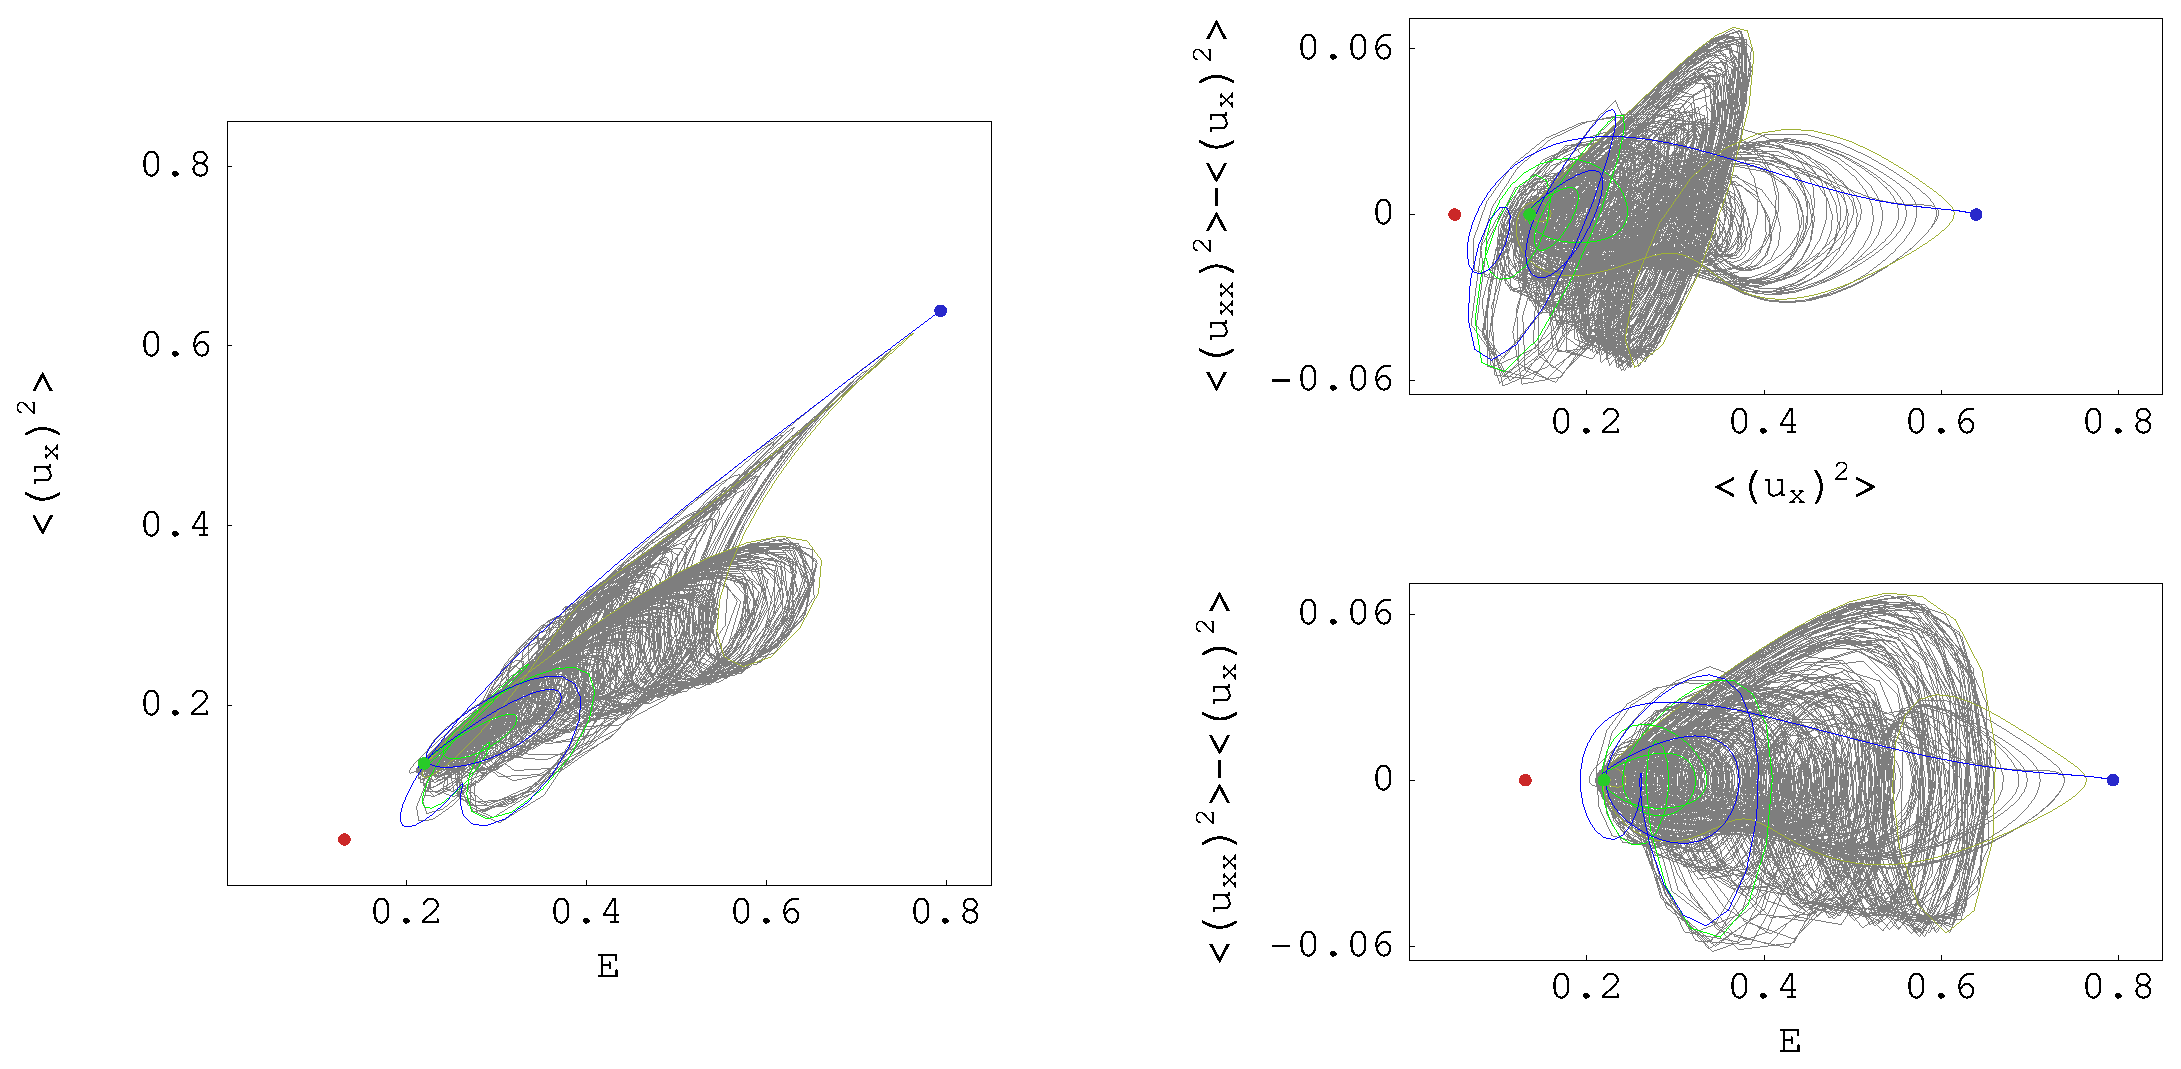
\includegraphics[width=0.8\textwidth]{figs/ks22TurbConn_xfig.eps}
\end{center}
\caption{
\EQV{1} (red), \EQV{2} (green), \EQV{3} (blue), 
connections from \EQV{1} to $A(L/4)\EQV{1}$ (green),
from $A(L/4)\EQV{1}$ to \EQV{1} (yellow-green) 
and from \EQV{3} to $A(L/4)\EQV{1}$ (blue), along
with a generic long-time ``turbulent" evolution (grey) for $L=22$. 
Three different projections of the 
$(E,\, \expct{(u_{x})^2},\, \expct{(u_{xx})^2})-\expct{(u_{x})^2})$
representation are shown.
        }
\label{f:drivedragConn}
\end{figure}
%%%%%%%%%%%%%%%%%%%%%%%%%%%%%%%%%%%%%%%%%%%%%%%%%%%%%%%%%%%%%%%%%%

% \PC{this is special to the $L=22$ system; eventually move to
%    the appropriate section}
\PC{ks22TurbConn2\_xfig.eps for \reffig{f:drivedragConn}
    not checked in?}
In \reffig{f:drivedrag}
we plot the power input $\expct{(u_{x})^2}$ vs.
dissipation $\expct{(u_{xx})^2}$ for all $L=22$ \eqva\ and
\reqva\ \PCedit{determined so far},
several \po s and \rpo s, and for a typical ``turbulent"
evolution.
% Notice that the single \rpo\ with $T\simeq32$ captures a large
% part of the turbulent dynamics
% \ES{Momentarilly adopting Japanese philosophy,
% before putting there the rest of the short orbits.}.
\PC{Re \reffig{f:drivedrag}:
%    (0) replace $y$-axis by
%    $\expct{(u_{xx})^2}-\expct{(u_{x})^2}$, so all \po s lie
%    on the $x$-axis and on can see more clearly the turbulent and
%    periodic trajectory, instead having them scrunched into the
%    diagonal. (a) Replace by side views of
%    3-$d$ $(\expct{u^2},\expct{(u_{x})^2},\expct{(u_{xx})^2}
%       -\expct{(u_{x})^2})$,
%    two figures; 
    (b) current type figure, with chaotic trajectory,
    all \eqva, $(32.\cdots,11)$ as example of well embedded, and
    a typical \po\ {\em not} embedded into the ``turbulent" attractor.
    (c) a separate figure with more \po s, no ``turbulent" attractor.
%    (d) prepare a mathematica macro that automatically uses
%    fonts at least twice the size you use currently. 
    (e) replace
    gray window with a white background, black font. (f) in the
    publication version replace colored dots with symbols of varying
    shapes, fine black border, can be filled in with colors.
    }
%\PC{In \reffig{f:drivedrag}:
%    do also try plotting the heteroclinic connections - they are
%    presumably off the diagonal
%   }
\PC{believe it or not, we are now set to compute
    $\timeAver{u^2}$ and $\timeAver{(u_x)^2}$
    using cycle expansions
    }

%%%%%%%%%%%%%%%%%%%%%%%%%%%%%%%%%%%%%%%%%%%%%%%%%%%%%%%%%%%%%%%%
\begin{figure}[t] \label{f:drivedragPoinc}
\begin{center}
    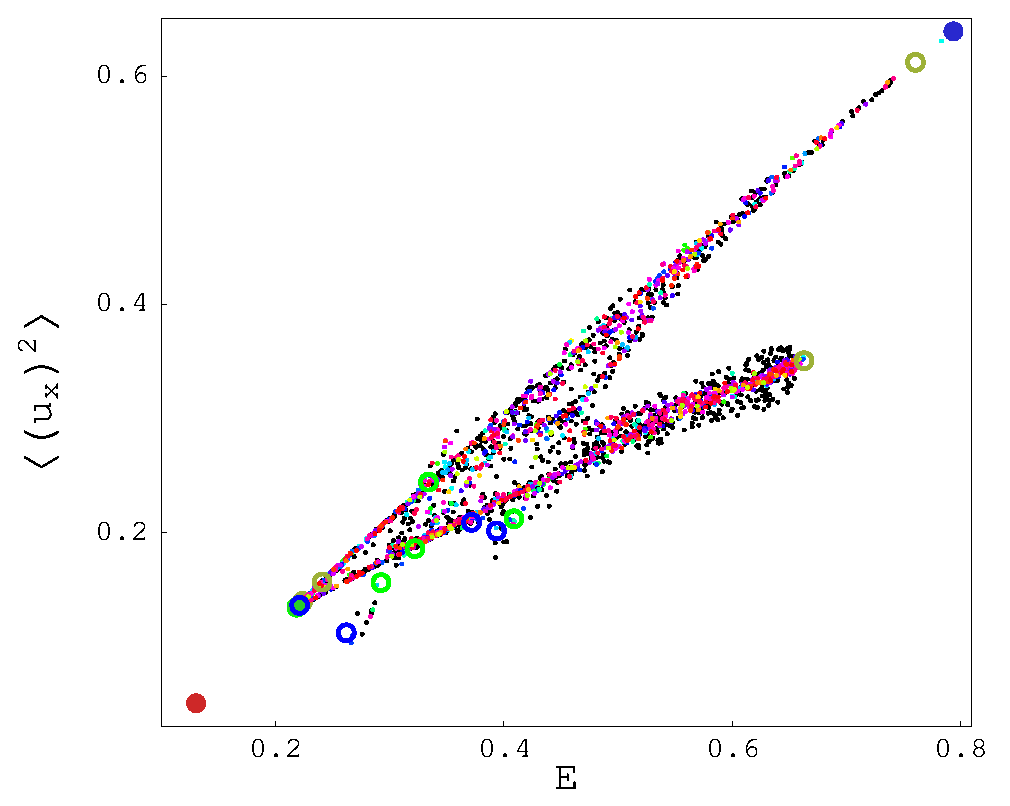
\includegraphics[width=0.8\textwidth]{figs/energyPoinc.eps}
\end{center}
\caption{
Shown on Poincar\'{e} surface of section $\expct{(u_{xx})^2} = \expct{(u_{x})^2}$:
\EQV{1}, \EQV{2} and \EQV{3} in red, green and blue solid points respectively,
connections from \EQV{1} to $A(L/4)\EQV{1}$,
from $A(L/4)\EQV{1}$ to \EQV{1} and from \EQV{3} to $A(L/4)\EQV{1}$ in green, 
yellow-green and blue circles respectively,
a typical ``turbulent" evolution (black) and all \po s and \rpo s 
determined so far for $L=22$.
        }
\end{figure}
%%%%%%%%%%%%%%%%%%%%%%%%%%%%%%%%%%%%%%%%%%%%%%%%%%%%%%%%%%%%%%%%%%


The time averaged energy density  $\timeAver{E}$
computed on a typical orbit goes to a constant, so
the expectation values \refeq{rpo:EtimAve} of drive and dissipation
exactly balance each out:
\beq
    \timeAver{\dot{E}}  =
    \lim_{t\rightarrow \infty}
        {1\over t} \int_0^t d\tau \, \dot{\expctE}
=
      \timeAver{(u_{x})^2} - \timeAver{(u_{xx})^2}
= 0
    \,.
\ee{rpo:EtimAve}
In particular, the \eqva\
and \reqva\ sit on the diagonal in \reffig{f:drivedrag},
and so do time averages computed on \po s and \rpo s:
\bea
\timeAver{E}_p &=&
{1\over \period{p}} \int_0^\period{p}d\tau \, \expctE(\tau)
    \continue
\timeAver{(u_{x})^2}_p &=&
{1\over \period{p}} \int_0^\period{p} d\tau \, \expct{(u_{x})^2}
    =
      \timeAver{(u_{xx})^2}_p
    \,.
\label{poE}
\eea

In the Fourier basis \refeq{EFourier} the conservation of energy on average
takes form
\beq
0 = \sum_{k=1}^{+\infty} ( (k/\tildeL)^2 - ( k/\tildeL)^4 )\,
    \timeAver{E_k}
\,,\qquad
E_k(t) =  |a_k(t)|^2
\,.
\ee{EFourier1}
The large $k$ convergence of this series is insensitive to the
system size $L$; $\timeAver{E_k}$ have to decrease much faster than
$1/( k/\tildeL)^4$.
\PC{determine the decay rate, presumably exponential in $k$}
Deviation of $E_k$ from this bound for small $k$ determines the active modes.
This may be useful to bound the number of equilibria, with
the upper bound given by zeros of a small number
of long wavelength modes.
For \eqva\ the $L$-independent bound
    on $E$ is given by Michaelson\rf{Mks86}. 
The best current bound\cite{GiacoOtto05,bronski-2005} on thge long-time limit
of $E$
as a function of the system size $L$ scales as 
$E \propto L^{3/2}$.
%
\PC{
 % Past: Michael Loss has not taught us how to bound $E$ by
 %  Sobolev bounds. Neither has Spiegel. Next: But 
  Constantin says that the answer is in
    \refrefs{temam85ks}. . Eckmann: the  best bound is by Otto\cite{GiacoOtto05}; the
    only bound close to k=0, better in essential way. See also \refref{bronski-2005}.
    Eckmann had $L^{8/5}$, but conceptually Otto is the best.
    When the solution is big, how long can it stay big? They found it cannot stay big for
    long. 
       }
\PC{Next for fluid guys: read Lieb and Ruelle to learn
    how to bound $E$ for plane Couette by Sobolev bounds}

